
% ----------------------------
% Slide: Tổng quan kiểm thử thành phần
% ----------------------------
\begin{frame}[t,fragile]
\frametitle{Tổng quan kiểm thử thành phần}
\begin{itemize}
    \item \textbf{Mục đích:} Xác nhận từng thành phần hệ thống hoạt động đúng thiết kế trước khi đánh giá hiệu năng tổng thể.
    \item \textbf{Các thành phần kiểm thử:}
    \begin{itemize}
        \item Module cảm biến đeo (4G/GPS)
        \item Khởi tạo hệ thống và kết nối mạng (Wi-Fi)
        \item Kết nối MQTT và truyền dữ liệu
        \item Phát hiện té ngã và xử lý cảnh báo
        \item Module Camera và truyền hình ảnh
        \item Xử lý nhận diện hình ảnh (Python)
        \item Đánh giá thực nghiệm cảm biến MPU, GPS
        \item Kênh cảnh báo Asterisk và Telegram
    \end{itemize}
\end{itemize}
\end{frame}

% ----------------------------
% Slide: Kiểm thử Module 4G/GPS
% ----------------------------
\begin{frame}[t,fragile]
\frametitle{Kiểm thử Module 4G/GPS}
\begin{itemize}
    \item \textbf{Mục đích:} Xác nhận khả năng giao tiếp AT command, kết nối 4G, thu nhận GPS.
    \item \textbf{Quy trình:}
    \begin{enumerate}
        \item Khởi tạo UART, kiểm tra modem và SIM.
        \item Đánh giá chất lượng sóng (\texttt{+CSQ}).
        \item Cấu hình APN, kích hoạt PDP context.
        \item Bật GPS và truy vấn tọa độ.
    \end{enumerate}
    \item \textbf{Log tiêu biểu:}
    \begin{minted}[fontsize=\footnotesize,breaklines]{text}
I (28339) SIM_4G: Received: +QIACT: 1,1,1,"9.204.251.200"
I (34349) SIM_4G: Received: +QGPSLOC: 10.88862,106.77975
    \end{minted}
    \item \textbf{Kết luận:} Module hoạt động ổn định, đảm bảo gửi cảnh báo và thông tin định vị.
\end{itemize}
\end{frame}

% ----------------------------
% Slide: Khởi tạo hệ thống & Kết nối mạng
% ----------------------------
\begin{frame}[t,fragile]
\frametitle{Khởi tạo hệ thống \& Kết nối mạng}
\begin{itemize}
    \item \textbf{Mục đích:} Xác nhận các module SIM4G-GPS, Wi-Fi và các tác vụ chính hoạt động bình thường.
    \item \textbf{Log tiêu biểu:}
    \begin{minted}[fontsize=\footnotesize,breaklines]{text}
I (9961) SIM4G_AT: Initializing SIM4G AT driver...
I (10011) APP_MAIN: System initialization complete.
I (10021) APP_MAIN: Application started successfully
    \end{minted}
    \item \textbf{Kết luận:} Hệ thống khởi tạo thành công, tích hợp phần mềm và phần cứng ổn định.
\end{itemize}
\end{frame}

% ----------------------------
% Slide: Kiểm thử MQTT
% ----------------------------
\begin{frame}[t,fragile]
\frametitle{Kiểm thử MQTT và truyền dữ liệu}
\begin{columns}[T]
    \column{0.55\textwidth}
    \begin{itemize}
        \item \textbf{Mục đích:} Kiểm tra kết nối broker MQTT và gửi bản tin định kỳ.
        \item \textbf{Log tiêu biểu:}
        \begin{minted}[fontsize=\footnotesize,breaklines]{text}
I (19961) USER_MQTT: MQTT_EVENT_CONNECTED
I (39991) JSON_WRAPPER: Created status payload:
{"device_id":"ESP32_DEV_76E48B","fall_detected":false,...}
        \end{minted}
        \item \textbf{Kết luận:} Kết nối MQTT ổn định, đảm bảo truyền dữ liệu tới hệ thống giám sát.
    \end{itemize}
    \column{0.45\textwidth}
    \begin{figure}
        \centering
        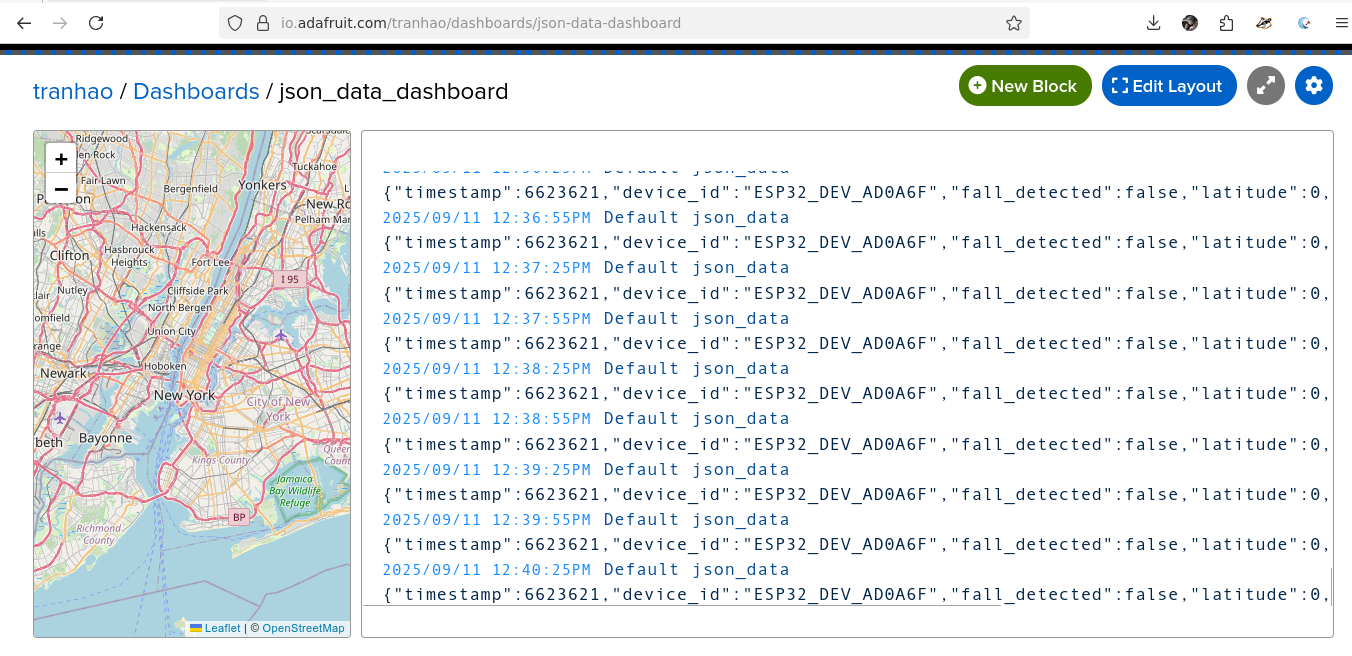
\includegraphics[width=\linewidth]{json_data_dashboard.png}
        \caption{Dashboard hiển thị bản tin MQTT.}
    \end{figure}
\end{columns}
\end{frame}

% ----------------------------
% Slide: Phát hiện té ngã & cảnh báo
% ----------------------------
\begin{frame}[t,fragile]
\frametitle{Phát hiện Té ngã \& Xử lý Cảnh báo}
\begin{columns}[T]
    \column{0.55\textwidth}
    \begin{itemize}
        \item \textbf{Quy trình:}
        \begin{enumerate}
            \item Thuật toán ghi nhận chuỗi trạng thái \texttt{LOW\_G} $\to$ \texttt{HIGH\_G}.
            \item Kích hoạt cảnh báo: SMS, MQTT, buzzer, LED.
        \end{enumerate}
        \item \textbf{Log thực tế:}
        \begin{minted}[fontsize=\footnotesize,breaklines]{text}
E (159131) FALL_LOGIC: FALL DETECTED! Accel: 0.99 g
I (159151) SIM4G_GPS: SMS request queued successfully
I (159881) SIM4G_AT: SMS sent successfully.
        \end{minted}
        \item \textbf{Kết luận:} Hệ thống phát hiện và xử lý cảnh báo thành công, đa kênh.
    \end{itemize}
    \column{0.45\textwidth}
    \begin{figure}
        \centering
        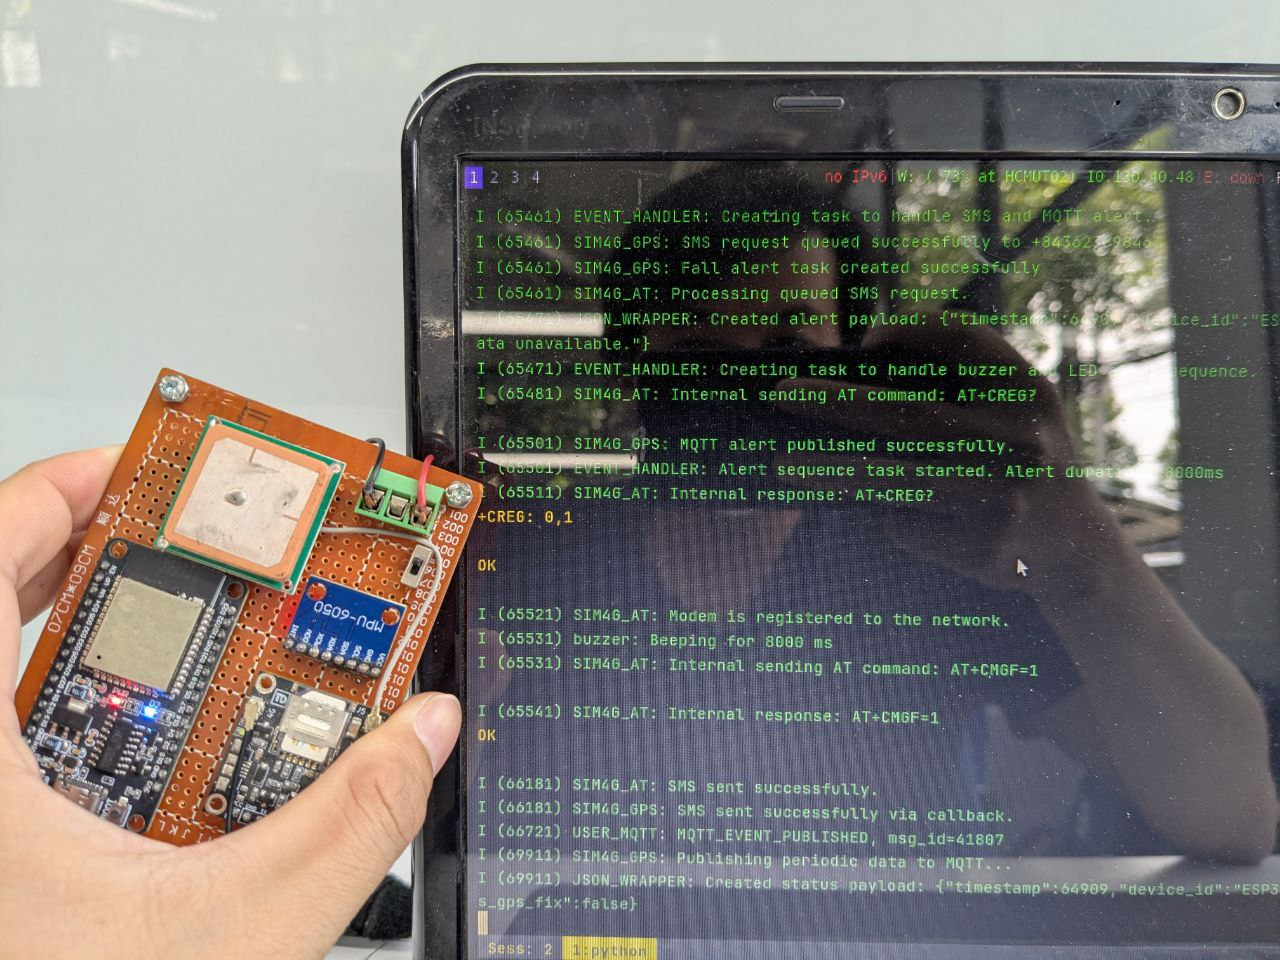
\includegraphics[width=\linewidth]{module1_real_log.jpg}
        \caption{Log thực tế module cảm biến đeo khi phát hiện té ngã.}
    \end{figure}
\end{columns}
\end{frame}

% ----------------------------
% Slide: Module Camera ESP32-CAM
% ----------------------------
\begin{frame}[t,fragile]
\frametitle{Kiểm thử Module Camera (ESP32-CAM)}
\begin{itemize}
    \item \textbf{Mục đích:} Xác nhận kết nối Wi-Fi và phát luồng hình ảnh qua HTTP.
    \item \textbf{Log tiêu biểu:}
    \begin{minted}[fontsize=\footnotesize,breaklines]{text}
I (9266) camera: Detected OV5640 camera
I (10006) esp32cam: HTTP server started
I (20006) esp32cam: Frames sent: 50, FPS: 5.87
    \end{minted}
    \item \textbf{Kết quả:} FPS trung bình 3.5–5, ổn định.
    \item \textbf{Kết luận:} Module camera hoạt động ổn định, giám sát trực tiếp.
\end{itemize}
\end{frame}

% ----------------------------
% Slide: Luồng hình ảnh Camera
% ----------------------------
\begin{frame}[t]
\frametitle{Luồng hình ảnh từ Camera}
\begin{figure}
    \centering
    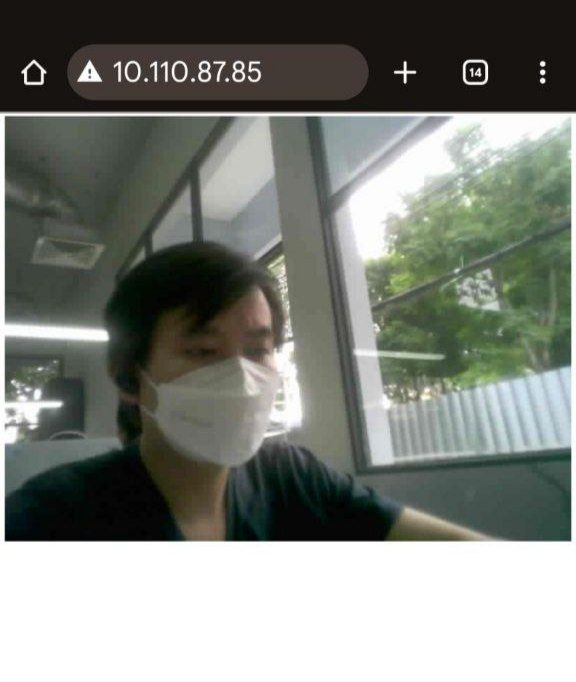
\includegraphics[width=0.85\linewidth]{module2_stream_example.jpg}
    \caption{Luồng hình ảnh phát từ module ESP32-CAM qua HTTP.}
\end{figure}
\end{frame}

% ----------------------------
% Slide: Xử lý nhận diện hình ảnh (Python)
% ----------------------------
\begin{frame}[t]
\frametitle{Xử lý nhận diện hình ảnh (Python)}
\begin{itemize}
    \item \textbf{Mục đích:} Xử lý luồng video, phát hiện người, trích xuất skeleton.
    \item \textbf{Quy trình:}
    \begin{itemize}
        \item Nhận luồng video từ ESP32-CAM.
        \item Tiền xử lý khung hình.
        \item TensorFlow Lite phát hiện người và vẽ skeleton.
    \end{itemize}
    \item \textbf{Kết quả:} Hoạt động ổn định, xử lý thời gian thực 3–5 FPS.
\end{itemize}
\end{frame}

% ----------------------------
% Slide: Kết quả xử lý hình ảnh
% ----------------------------
\begin{frame}[t]
\frametitle{Kết quả xử lý hình ảnh}
\begin{figure}
    \centering
    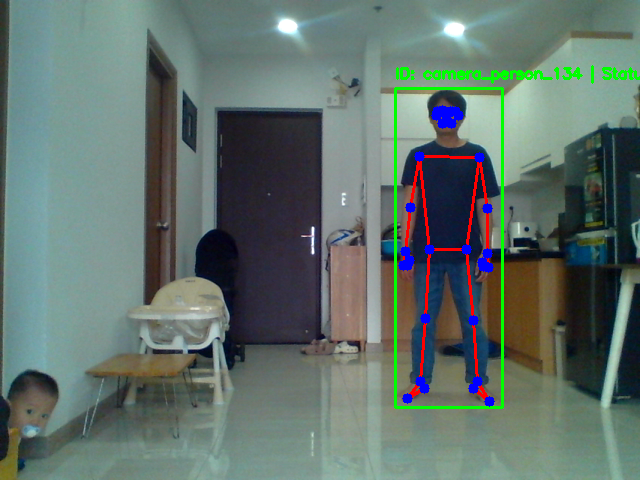
\includegraphics[width=0.85\linewidth]{fall_detection_screen_shoot.png}
    \caption{Module Python phát hiện người và vẽ skeleton.}
\end{figure}
\end{frame}
  

%======================= ok doan nay =================%


% ----------------------------
% Slide: Log thực nghiệm Python
% ----------------------------
\begin{frame}[fragile]
\frametitle{Log thực nghiệm Python}
\begin{figure}[H]
    \centering
    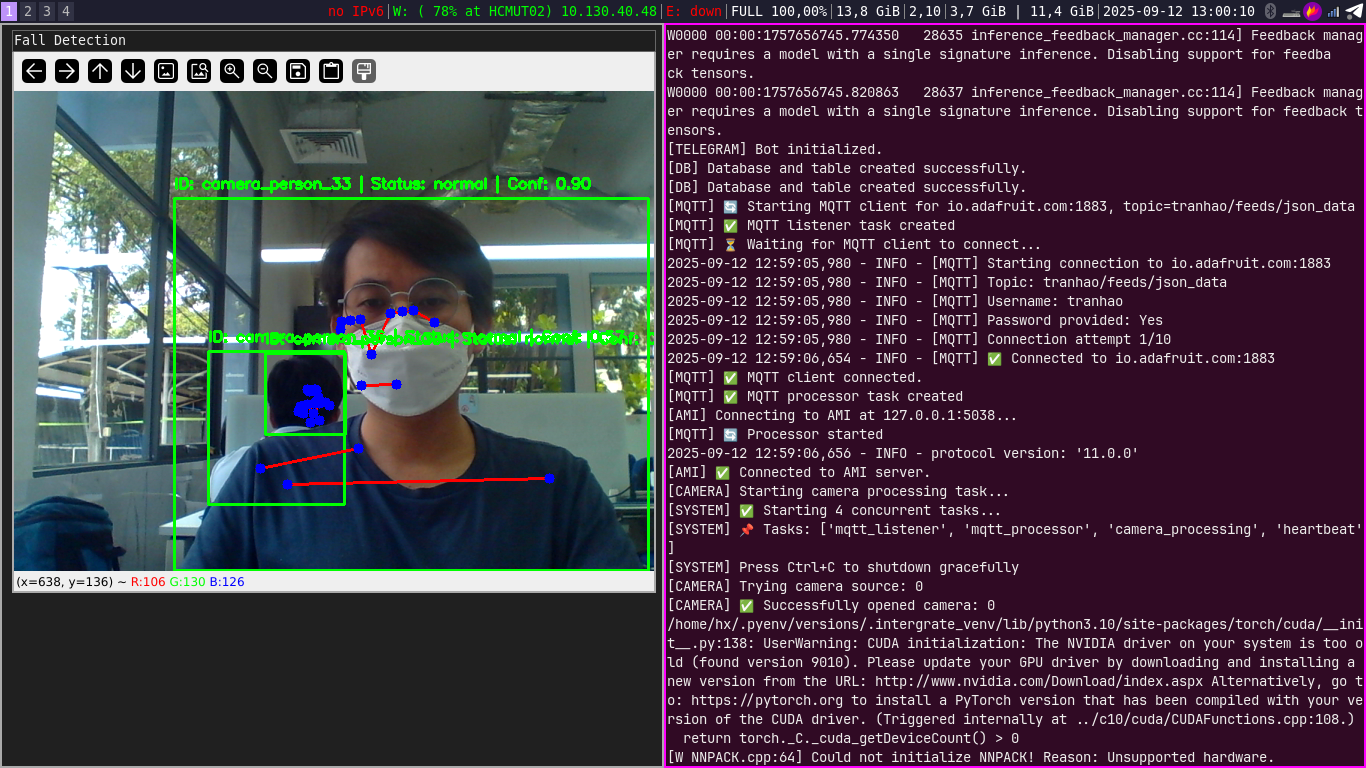
\includegraphics[width=0.85\linewidth]{python_runing_log.png}
    \caption{Log Python xử lý luồng camera và điều phối cảnh báo.}
\end{figure}
\begin{itemize}
    \item \textbf{Kết luận:} Module Python hoạt động ổn định, xử lý dữ liệu camera, đồng bộ MQTT và kích hoạt cảnh báo thành công.
\end{itemize}
\end{frame}

% ----------------------------
% Slide: Đánh giá dữ liệu cảm biến MPU6050
% ----------------------------
\begin{frame}[fragile]
\frametitle{Đánh giá dữ liệu cảm biến (MPU6050)}
\begin{itemize}
    \item \textbf{Quy trình:} Giả lập té ngã, so sánh dữ liệu cảm biến giữa \textbf{bình thường} và \textbf{té ngã}.
    \item \textbf{Kết quả:}
    \begin{itemize}
        \item \textbf{Gyro (dps):} Bình thường $\approx \pm 1.5$ dps; té ngã tăng vọt $\approx \pm 250$ dps.
        \item \textbf{Accel (g):} Bình thường $\approx 0.93$ g; té ngã dao động $-2.0$ g đến $+1.0$ g.
    \end{itemize}
    \item \textbf{Kết luận:} \textbf{Accel\_Mag} và \textbf{Gyro\_Mag} là chỉ báo hiệu quả để phát hiện té ngã.
\end{itemize}
\end{frame}

% ----------------------------
% Slide: Biến thiên Gyro_Mag
% ----------------------------
\begin{frame}[fragile]
\frametitle{Biến thiên dữ liệu Gyro\_Mag}
\begin{figure}[H]
    \centering
    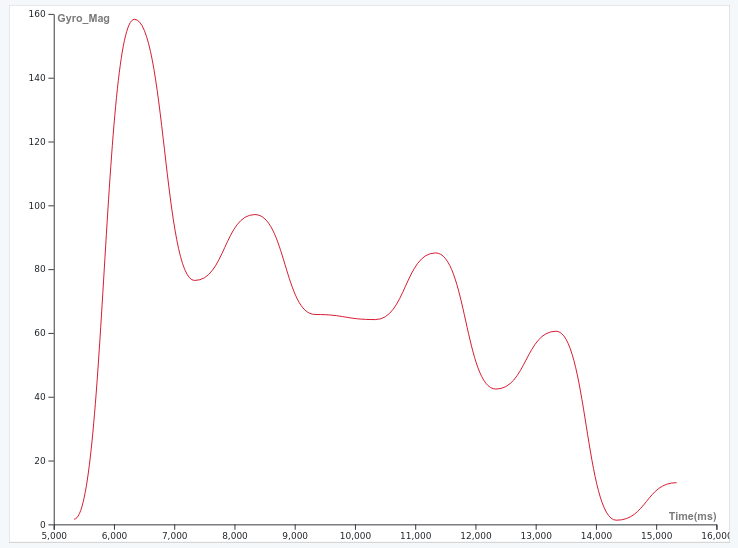
\includegraphics[width=0.95\linewidth]{gyro_time.png}
    \caption{Biến thiên magnitude của gia tốc góc (Gyro\_Mag) theo thời gian.}
\end{figure}
\end{frame}

% ----------------------------
% Slide: Phân tích đồ thị Gyro_Mag
% ----------------------------
\begin{frame}[fragile]
\frametitle{Phân tích Gyro\_Mag}
\begin{itemize}
    \item \textbf{Bình thường (Normal):} Dao động nhỏ quanh giá trị nền ($\lesssim 2$ dps).
    \item \textbf{Sự kiện té ngã (Fall):} Xuất hiện đỉnh lớn (hàng chục đến hàng trăm dps) do va chạm mạnh.
    \item \textbf{Hậu té (Post-Fall):} Giảm nhanh về mức nền, thể hiện trạng thái nằm yên.
\end{itemize}
\end{frame}

% ----------------------------
% Slide: Biến thiên Accel_Mag
% ----------------------------
\begin{frame}[fragile]
\frametitle{Biến thiên dữ liệu Accel\_Mag}
\begin{figure}[H]
    \centering
    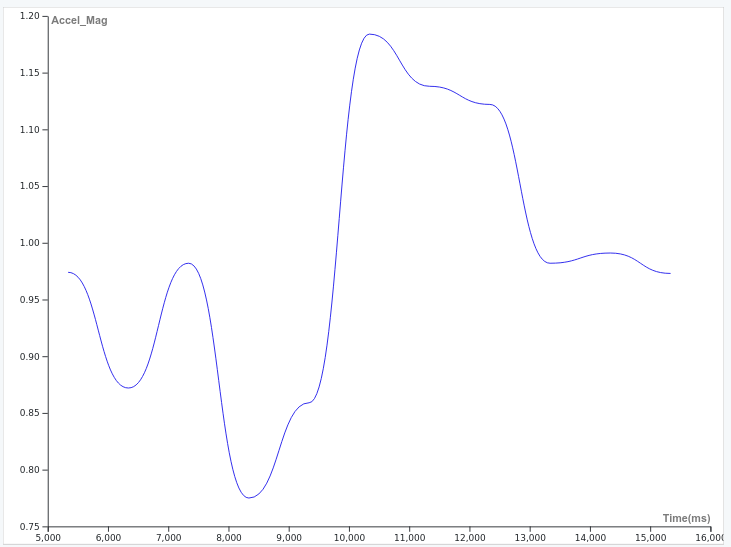
\includegraphics[width=0.95\linewidth]{accel_time.png}
    \caption{Biến thiên magnitude của gia tốc (Accel\_Mag) theo thời gian.}
\end{figure}
\end{frame}

% ----------------------------
% Slide: Phân tích đồ thị Accel_Mag
% ----------------------------
\begin{frame}[fragile]
\frametitle{Phân tích Accel\_Mag}
\begin{itemize}
    \item \textbf{Bình thường (Normal):} Nằm gần 1\,g.
    \item \textbf{Sự kiện té ngã (Fall):} Xuất hiện xung hoặc thay đổi đột ngột, vượt hoặc giảm mạnh so với 1\,g.
    \item \textbf{Hậu té (Post-Fall):} Trở về gần 1\,g nhưng phân bố vector khác (tư thế nằm).
\end{itemize}
\end{frame}

% ----------------------------
% Slide: Kiểm thử cảnh báo Asterisk AMI
% ----------------------------
\begin{frame}[fragile]
\frametitle{Kiểm thử cảnh báo qua Asterisk AMI}
\begin{itemize}
    \item \textbf{Mục đích:} Kiểm chứng cuộc gọi và SMS tự động.
    \item \textbf{Kết quả:}
    \begin{itemize}
        \item Kết nối thành công tới Asterisk AMI.
        \item SMS tới \texttt{6001} và \texttt{6002} thành công; \texttt{6003} lỗi.
        \item Một số lỗi gọi điện do không có thoại, không ảnh hưởng đến cảnh báo chính.
    \end{itemize}
\end{itemize}
\begin{figure}[H]
    \centering
    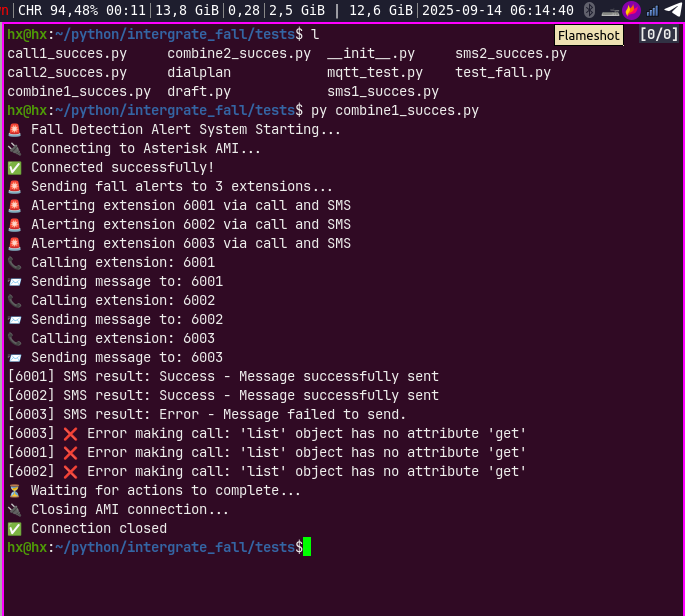
\includegraphics[width=0.95\linewidth]{ast_call_sms_test.png}
    \caption{Kết quả thử nghiệm chức năng gọi và nhắn tin qua Asterisk AMI.}
\end{figure}
\end{frame}

% ----------------------------
% Slide: Kiểm thử cảnh báo Telegram
% ----------------------------
\begin{frame}[fragile]
\frametitle{Kiểm thử cảnh báo qua Telegram}
\begin{itemize}
    \item \textbf{Cơ chế hoạt động:}
    \begin{itemize}
        \item \textbf{Từ phần cứng:} MQTT từ thiết bị -> hệ thống trung tâm -> Telegram.
        \item \textbf{Từ Python:} Camera -> Python gửi cảnh báo trực tiếp đến Telegram kèm hình ảnh.
    \end{itemize}
\end{itemize}
\end{frame}

% ----------------------------
% Slide: Thông báo Telegram từ phần cứng
% ----------------------------
\begin{frame}[fragile]
\frametitle{Thông báo Telegram (Phần cứng)}
\begin{figure}[H]
    \centering
    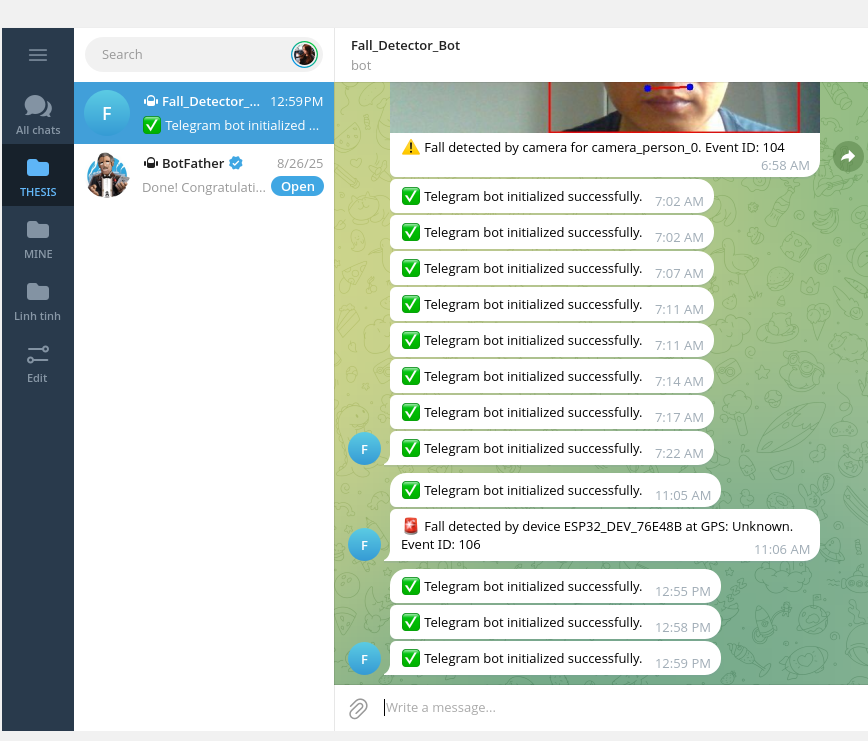
\includegraphics[width=0.8\linewidth]{telegram_fall_module1_send.png}
    \caption{Thông báo té ngã từ phần cứng qua Telegram.}
\end{figure}
\end{frame}

% ----------------------------
% Slide: Thông báo Telegram từ Python
% ----------------------------
\begin{frame}[fragile]
\frametitle{Thông báo Telegram (Python)}
\begin{figure}[H]
    \centering
    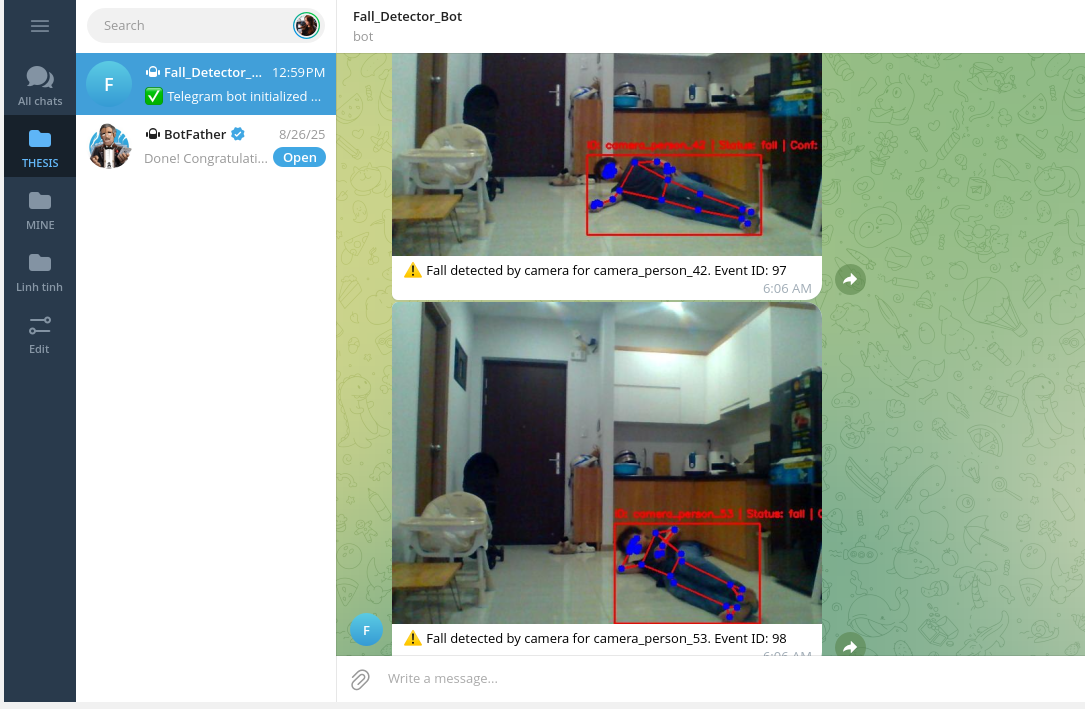
\includegraphics[width=0.8\linewidth]{telegram_python_fall_send.png}
    \caption{Thông báo té ngã từ module Python qua Telegram.}
\end{figure}
\begin{itemize}
    \item \textbf{Kết luận:} Kênh Telegram hoạt động ổn định, kết hợp cả hai nguồn cảnh báo tăng độ tin cậy.
\end{itemize}
\end{frame}
